\documentclass[10pt,letterpaper,twocolumn]{article}

%%% PREAMBLE %%%
\usepackage{amsmath}
%\usepackage{amsthm}
%\usepackage{amssymb}
%\usepackage{booktabs}
%\usepackage{tabularx}
%\usepackage{subfigure}
\usepackage{mathrsfs}
\usepackage{textcomp}
\usepackage{siunitx}
\usepackage{hyperref}
\usepackage{multirow}
\usepackage{empheq}
\usepackage{calc}
\usepackage[version=3]{mhchem}
\usepackage{tikz}
\usepackage{pgfplots}
\usepackage{xcolor}
\usepackage[section]{placeins}
\pgfplotsset{compat=newest}


\hypersetup{
 colorlinks=false,
 linkbordercolor={1 1 1},
 citebordercolor={1 1 1},
 urlbordercolor={1 1 1} 
}

\sisetup{ 
% load-configurations=abbreviations
% round-mode = places,
}%

% New definition of square root:
% it renames \sqrt as \oldsqrt
% This definition puts a little vertical guy at the end so it's more
% obvious where the square root actually ends.
\let\oldsqrt\sqrt
% it defines the new \sqrt in terms of the old one
\def\sqrt{\mathpalette\DHLhksqrt}
\def\DHLhksqrt#1#2{%
\setbox0=\hbox{$#1\oldsqrt{#2\,}$}\dimen0=\ht0
\advance\dimen0-0.2\ht0
\setbox2=\hbox{\vrule height\ht0 depth -\dimen0}%
{\box0\lower0.4pt\box2}}

% integrals with infinity bounds
\newcommand{\intinfty}{\int_{-\infty}^{\infty}}

% consistent formatting of object labels
\newcommand{\Figure}[1]{FIG. \ref{#1}}
\newcommand{\Equation}[1]{Equation \ref{#1}}
\newcommand{\Table}[1]{TBL. \ref{#1}}
\newcommand{\Section}[1]{SEC. \ref{#1}}
\newcommand{\Chapter}[1]{CH. \ref{#1}}
\newcommand{\Appendix}[1]{APP. \ref{#1}}

% missing mathematical operators
\DeclareMathOperator{\sinc}{sinc}
\DeclareMathOperator{\sech}{sech}
\DeclareMathOperator{\sgn}{sgn}
\DeclareMathOperator{\erf}{erf}
\DeclareMathOperator{\inverf}{inverf}
\DeclareMathOperator{\arcsinh}{arcsinh}
\DeclareMathOperator{\arccosh}{arccosh}
\DeclareMathOperator{\arctanh}{arctanh}

% use roman type for natural base e and sqrt(-1)
\newcommand{\me}{{\mathrm{e}}}
\newcommand{\mi}{{\mathrm{i}}}

% roman type for the derivative, plus a space
\newcommand{\md}{\,\mathrm{d}}

% fourier transform and the reverse
\newcommand{\ff}[1]{{\mathscr{F}^{+}\bigl(#1\bigr)}}
\newcommand{\fr}[1]{{\mathscr{F}^{-}\bigl(#1\bigr)}}

% hilbert transform and the reverse
\newcommand{\hf}[1]{{\mathscr{H}^{+}\bigl(#1\bigr)}}
\newcommand{\hr}[1]{{\mathscr{H}^{-}\bigl(#1\bigr)}}

% custom colors for 2D plots - these are the same ones mathematica uses by
% default

% color
%\definecolor{colora}{RGB}{63,61,153}
%\definecolor{colorb}{RGB}{153,61,113}
%\definecolor{colorc}{RGB}{153,139,61}

% black and white
\definecolor{colora}{RGB}{70,70,70}
\definecolor{colorb}{RGB}{70,70,70}
\definecolor{colorc}{RGB}{70,70,70}
\definecolor{coloraa}{RGB}{0,0,0}
\definecolor{colorbb}{RGB}{0,0,0}
\definecolor{colorcc}{RGB}{0,0,0}

% display units on plots
\usepgfplotslibrary{units}
\usetikzlibrary{pgfplots.units} 

%%% END PREAMBLE %%%

\begin{document}
\thispagestyle{empty}
\pgfplotsset{
 minor tick num=3,
 small,
 every axis/.style={thick,width=0.55\textwidth,height=0.20\textwidth},
 legend pos = north east,
 axis on top,
 normalise/.style 2 args={
  scaled x ticks=manual:{}{% 
   \pgfmathparse{ ( ##1 - (#1) ) }%
  }
 }
}
\begin{tabular}{cc}
$z=\SI{10}{\micro\meter}$ & $z=\SI{10}{\micro\meter}$ \\
\begin{tikzpicture}[baseline,trim axis left]
 \begin{axis}[restrict x to domain=31:100,normalise={30}{30}]
\addplot[color=coloraa] file {data/2-norm.dat};
\addplot[color=colora,mark=o,mark size={1.500},only marks,mark repeat=3]
file {data/near02-line-mod-norm.txt};
%\addlegendentry{$z=\SI{10}{\micro\meter}$}
\node[anchor=base east] at (0.430\textwidth,-0.009\textwidth)
{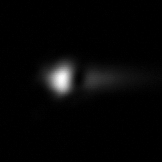
\includegraphics[height=0.11\textwidth,keepaspectratio]{images/bw/123-11.png}};
%\addplot graphics [xmin=60,xmax=80,ymin=-0.01,ymax=0.4] {images/bw/321-1.png};
\end{axis}
\end{tikzpicture}%
&
\begin{tikzpicture}[baseline,trim axis right]
 \begin{axis}[restrict x to domain=-9:60,normalise={-10}{-10}]
\addplot[color=coloraa] file {data/2b-norm.dat};
\addplot[color=colora,mark=o,mark size={1.50},only marks,mark repeat=3]
file {data/conenear-line-mod-norm.txt};
\node[anchor=base east] at (0.430\textwidth,-0.009\textwidth)
{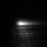
\includegraphics[height=0.11\textwidth,keepaspectratio]{images/bw/conenear.png}};
%\addlegendentry{$z=\SI{10}{\micro\meter}$}
\end{axis}
\end{tikzpicture}%
\\
$z=\SI{1.0}{\milli\meter}$ & $z=\SI{1.0}{\milli\meter}$ \\
\begin{tikzpicture}[baseline,trim axis left]
 \begin{axis}[restrict x to domain=475:725,normalise={500}{}]
\addplot[color=colorbb] file {data/3-norm.dat};
\addplot[color=colorb,mark=o,mark size={1.50},only marks,mark repeat=3]
file {data/midfield-line-mod-norm.txt};
\node[anchor=base east] at (0.430\textwidth,-0.009\textwidth)
{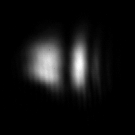
\includegraphics[height=0.11\textwidth,keepaspectratio]{images/bw/midfield.png}};
\end{axis}
\end{tikzpicture}%
&
\begin{tikzpicture}[baseline,trim axis right]
\begin{axis}[restrict x to domain=1100:1350,normalise={1100}{}]
\addplot[color=colorbb] file {data/3b1-norm.dat};
\addplot[color=colorb,mark=o,mark size={1.50},only marks,mark repeat=3]
file {data/conemid03-line-mod-norm.txt};
\node[anchor=base east] at (0.430\textwidth,-0.009\textwidth)
{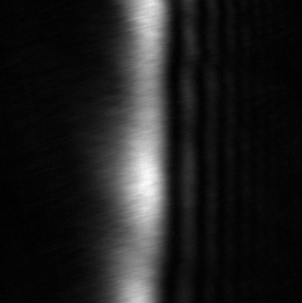
\includegraphics[height=0.11\textwidth,keepaspectratio]{images/bw/321-7.png}};
%\addlegendentry{$z=\SI{0.1}{\milli\meter}$}
\end{axis}
\end{tikzpicture}%
\\
$z=\SI{100}{\milli\meter}$ & $z=\SI{100}{\milli\meter}$ \\
\begin{tikzpicture}[baseline,trim axis left]
\begin{axis}[
xlabel=detector scale,
/pgfplots/change x base,
/pgfplots/x unit=\si{\micro\meter},
restrict x to domain=54000:68000,
normalise={54000}{},
]
\addplot[color=colorcc] file {data/5-norm.dat};
\addplot[color=colorc,mark=o,mark size={1.50},only marks,mark repeat=3]
file {data/farfield02-avg-mod-norm.txt};
%\addlegendentry{$z=\SI{100}{\milli\meter}$}
\node[anchor=base east] at (0.430\textwidth,-0.009\textwidth)
{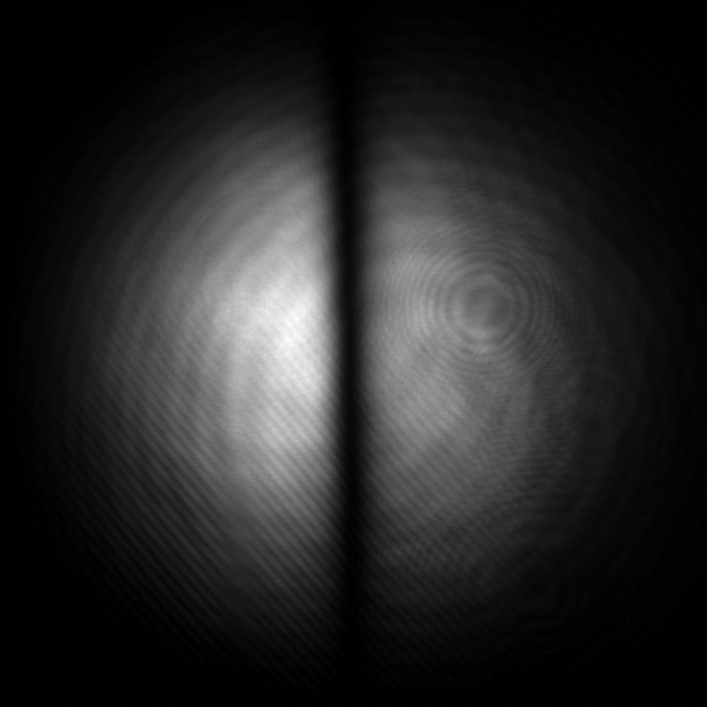
\includegraphics[height=0.11\textwidth,keepaspectratio]{images/bw/farfield02.png}};
\end{axis}
\end{tikzpicture}%
&
\begin{tikzpicture}[baseline,trim axis right]
\begin{axis}[
xlabel=detector scale,
/pgfplots/change x base,
/pgfplots/x unit=\si{\micro\meter},
restrict x to domain=54000:68000,
normalise={54000}{},
]
\addplot[color=colorcc] file {data/5b-norm.dat};
\addplot[color=colorc,mark=o,mark size={1.50},only marks,mark repeat=3]
file {data/farfield-cone-mod-norm.txt};
%\addlegendentry{$z=\SI{100}{\milli\meter}$}
\node[anchor=base east] at (0.430\textwidth,-0.009\textwidth)
{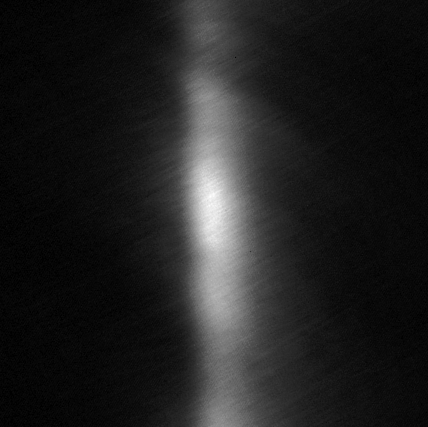
\includegraphics[height=0.11\textwidth,keepaspectratio]{images/bw/321-9.png}};
\end{axis}
\end{tikzpicture}%
\end{tabular}
\end{document}
% Fresnel Numbers:
% Lorentz-Drude Model -14.48239364+1.094554854i 1.744521043e-05
% octave:24> (1.744*10^-5)^2/((0.1*10^-3)*(632.8*10^-9))
% ans =  4.8065
% octave:25> (1.744*10^-5)^2/((100*10^-3)*(632.8*10^-9))
% ans =  0.0048065
% octave:26> (1.744*10^-5)^2/((10*10^-6)*(632.8*10^-9))
% ans =  48.065
